\chapter{Fundamental Interactions}
\label{chap:funda}
    \begin{tcolorbox} [colframe=blue!15!black,colback=yellow!29.05!white,arc=1em,fonttitle=\bfseries,title= Key Objectives:, width = \textwidth]
        $\star$ \textbf{Fundamental Interactions in Nature} $\star$
        \begin{itemize}
            \item Strong Interaction
            \item Weak Interaction
            \item Electro-Magnetic Interaction
            \item Gravitational Interaction
        \end{itemize}
       $\star$ \textbf{Force Carriers} $\star$ \\
       $\star$ \textbf{Feynman Diagram} $\star$
       
     \end{tcolorbox}
    
    \section{Fundamental Interactions}
 We may have experienced so many different types of forces around us but the amazing
simplifications in physics is that only four fundamental interactions can account for all known physical phenomena happening around us in the \href{https://en.m.wikipedia.org/wiki/Standard_Model}{{{Standard model}}}.
These four interactions have different ranges, different strengths and act in completely different time and mass scales. 
The summary of these four fundamental interactions are as follows: \\
  
\begin{table}[ht]
        \centering
        \begin{adjustbox}{width=1\textwidth}
        {\Large
        \begin{tabular}{|l|l|c|c|c|p{5cm}|}
            \hline
            \textbf{Interaction} & \textbf{Force Carrier} & \textbf{Relative Strength} & \textbf{Range(m)} & \textbf{Nature} & \textbf{Example}\\[0.5cm]
            \hline
              
            \textbf{Gravitational} & \textbf{\emph{Graviton}} & $10^{-38}$ & $\infty$ & \textbf{Attractive} & {Interaction due to mass} \\[1.25cm]
              
            \textbf{Electro-magnetic} & \textbf{\emph{Photon}} & $10^{-2}$ & $\infty$ & \textbf{Attractive/Repulsive} & {Interaction due to Charge} \\[1.25cm]
              
            \textbf{Weak} & \textbf{\emph{Vector Bosons} \newline ($W^\pm,Z^0$)} & $10^{-5}$ & $10^{-18}$ & \textbf{Attractive/Repulsive} & {Change of the flavour \newline of Quark i.e Beta-decay} \\[1.25cm]
              
            \textbf{Strong} & \textbf{\emph{Gluon}} & $1$ & $10^{-15}$ & \textbf{Attractive/Repulsive} & {Interaction between Quarks}\\[1.25cm]\hline
    
    \end{tabular}}
    \end{adjustbox}
\caption{Summary of fundamental interactions}
\label{tab:table_1}
\end{table}
    
    \par You must have been quite uncomfortable with so many new terms such as Quarks, Vector Bosons, Gluons and flavour. Don't worry we will learn about them in due course of time but for the time being let us concentrate only on the interactions.
    \pagebreak\begin{itemize}
          \item\textbf{The strong interaction} is the strongest among all the four. It acts over an extremely short range and thus loses its superiority beyond a few \textit{fermi}. It determines the stability of nuclei and thus relative abundance elements in nature. The properties of the nucleus also determines the number of electrons in it and therefore, indirectly controls the chemical reactions. It also determines the release of energy in nuclear reactions.
          \item\textbf{The Electro-magnetic interaction} is a combination of electric and magnetic force.(Till the beginning of the 19th century, these two were considered as two distinct forces. Riding on the series of works of various scientists between 1820 and 1873, James Maxwell formally unified these two seemingly different forces into one as electromagnetic interaction). It is a long-range force and it acts over extremely large distances. Though it is the second strongest interaction among the four and responsible for almost all phenomena(eg. friction, tension, chemical reactions and electrical effects) we experience in our daily lives. However, its often cancels out in the macroscopic body and becomes insignificant. However if it does not cancel, it would supersede the Gravitaional Force as expected.
          \pagebreak\item\textbf{The Gravitational interaction} is the weakest among the four partners and is always attractive. But it is interesting to note that it is the key interaction which determines the evolution of the universe once the matter is formed. In astronomical scale, it dominates over the other interactions and as we know it, governs the motions of the celestial objects. The gravitational force is also responsible for modifying the space and time near very massive bodies, such as stars and planets.
        \end{itemize}
        
    \section{Force Carrier/ Exchange Particles}
    One thing must have come to your mind, ``How can two particles interact with each other without any physical contact?'' or ``How does a charged particle know that there is(are) other charged particle(s) in another location(s)?"
    
    \par Here comes the concept of a force carrier. It was first proposed by Yukawa's in 1935 while working on the nuclear force.(Earlier, Heisenberg had applied the concept of exchange force to explain the formation of $H_2$ molecules through the binding of Hydrogen atoms.) Yukawa proposed that the interactions are transmitted by the exchange of elementary particles. Note that this concept complements the concept of force field. According to the force field concept, the interactions between two particles maybe described as a field generated by each particle which affects others due to the exchange of field quanta. When we quantize these  fields, it results in various excitation states and each state corresponds to a different generation of force carrier particles (we will discuss this ``different generation of force carrier particles", in the Fundamental particles section.) If not for the other interactions, the field is called the Electromagnetic Field and the particle is, Gluon. The other exchange particles for the other interactions are given in the above table. We will conclude this paragraph mentioning that these force carrier particles are considered as Virtual Particles. In the next paragraph, we will explore this term and see how we can even violate conservation of mass-energy principle. Yes! you hear it correctly. Let us start:
    
        \par {\textbf{Virtual Particle: } Suppose, you have a particle with energy $E$. The Heisenberg Uncertainty Principle states that this energy cannot be measured with any arbitrary accuracy. If you want to measure it with an accuracy of $∆E$, you need to make this measurement over a time interval greater than $\hbar/∆t $ (using $\Delta E \Delta t > \hbar $). So, we don't know what is happening within the time interval $\Delta t$. It is gone to the extent that even if we violate the well known mass-energy conservation by an amount $\Delta E $, then by no means anybody can detect this violation within the time gap $\Delta t $. Therefore, it is possible to create a temporary field quanta of mass m($=c^2/\Delta E$) for a time interval of $\Delta t $. These field quanta are called Virtual Particles as they don't live beyond $\Delta t $ and thus cannot be directly observed. However we can record their effects. }
         \par [
         \textbf{\underline{Note:}} \textit{Virtual particles are real particles. According to Quantum Mechanics, every particle spends some time as a combination of other particles in all possible ways. It is well established and tested. Though the virtual particles are temporary, they interact with real particles and leave their `fingerprint' which can be experimentally verified unambiguously. The first proof was the observation of the Lamb Shift in Hydrogen atom by Willis Lamb and fir which he won the Nobel Prize.}]
         
         \par{\textbf{Range of the Interaction:} The above concept also allows us to estimate the range of the interactions. We have learned that Exchange Particles or Field Quantas are temporary and exist only for $\Delta t $. We can extend it to another step as     \begin{equation}
                \Delta t = \hbar/ \Delta E = \hbar/mc^2
            \end{equation} 
         If we consider the exchange particles are massive, then heavier their mass, shorter their existence $\Delta t $. If we further assume their velocity is equal to speed of light $c$ then in time $\Delta t $, it can travel a distance $r_0$, called range.}
             \begin{equation}
             r_0 = c. \Delta t = c \hbar/mc^2 = \hbar /mc
             \end{equation}
         \par Let us look at the implication of this concept. We already know that the strong interaction is very short range and radius of any nucleus is order of few \textit{fm}. Then
         \begin{equation}
         \begin{split}
                    mc^2~\sim~\hbar c /r_0 = 197/2 (MeV~fm)/fm =100~MeV
                    \\\textrm (assuming~~r_0 \sim 2fm)
         \end{split}
         \end{equation}
        \par This way Yukawa predicted the mass of the Mesons ($\pi^\pm , \pi^0$ to be $~$100 MeV. Later it was found to be $~$139 MeV and if you agree this is remarkable.
        
        \begin{wrapfigure}{r}{0.45\textwidth}
        \centering
        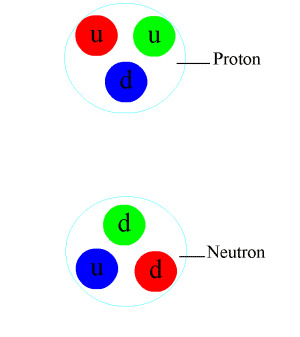
\includegraphics[width=0.3\textwidth]{02/nucleons.jpg}
        %\caption{\\Proton-neutron interaction}
        \label{fig:nucleons}
        \end{wrapfigure}
        
    Now you should realize why Electromagnetic Interaction is long range (infinite range). It is due to the fact that its exchange particle, Photon, is massless. This way we can predict the mass of the exchange particles if we know the range of the interactions or vice–versa. The attached animation (source: \href{https://en.wikipedia.org/wiki/Nuclear_force}{Wikipedia} ) portrays the interaction between a proton and a neutron through the exchange of a Meson.

    \par The process described above can also be visualized in pictorial form. It was first proposed by Richard Feynman. Though we have no intention to learn it in full glory which is beyond the scope of this class, we just like to get a taste of it. 
    
    \section{Feynman Diagram}
        \par We have learned that for each interaction there are virtual particles which exist only for $\Delta t $ time interval. Therefore, we can exploit this uncertainty to formulate a picture of the particle or particles in question in a space-time diagram. For sake of simplicity, we consider an electron at rest. If the electron emits a photon and absorb the same with a time interval of $\Delta t $, we won't be able to realise that. Such an event can be drawn as follows: 
        \par The Fermions are represented by a straight line with an arrow directing the flow of the particle. The photons are represented by a wavy line. The points where particles are created or annihilated are called Vertices. Here the line is vertical as the electron is at rest and only time is changing. During the time interval $\Delta t(= t_2–t_1)$, the virtual photon is created at $t_1$
        \begin{figure}
            \begin{center}
                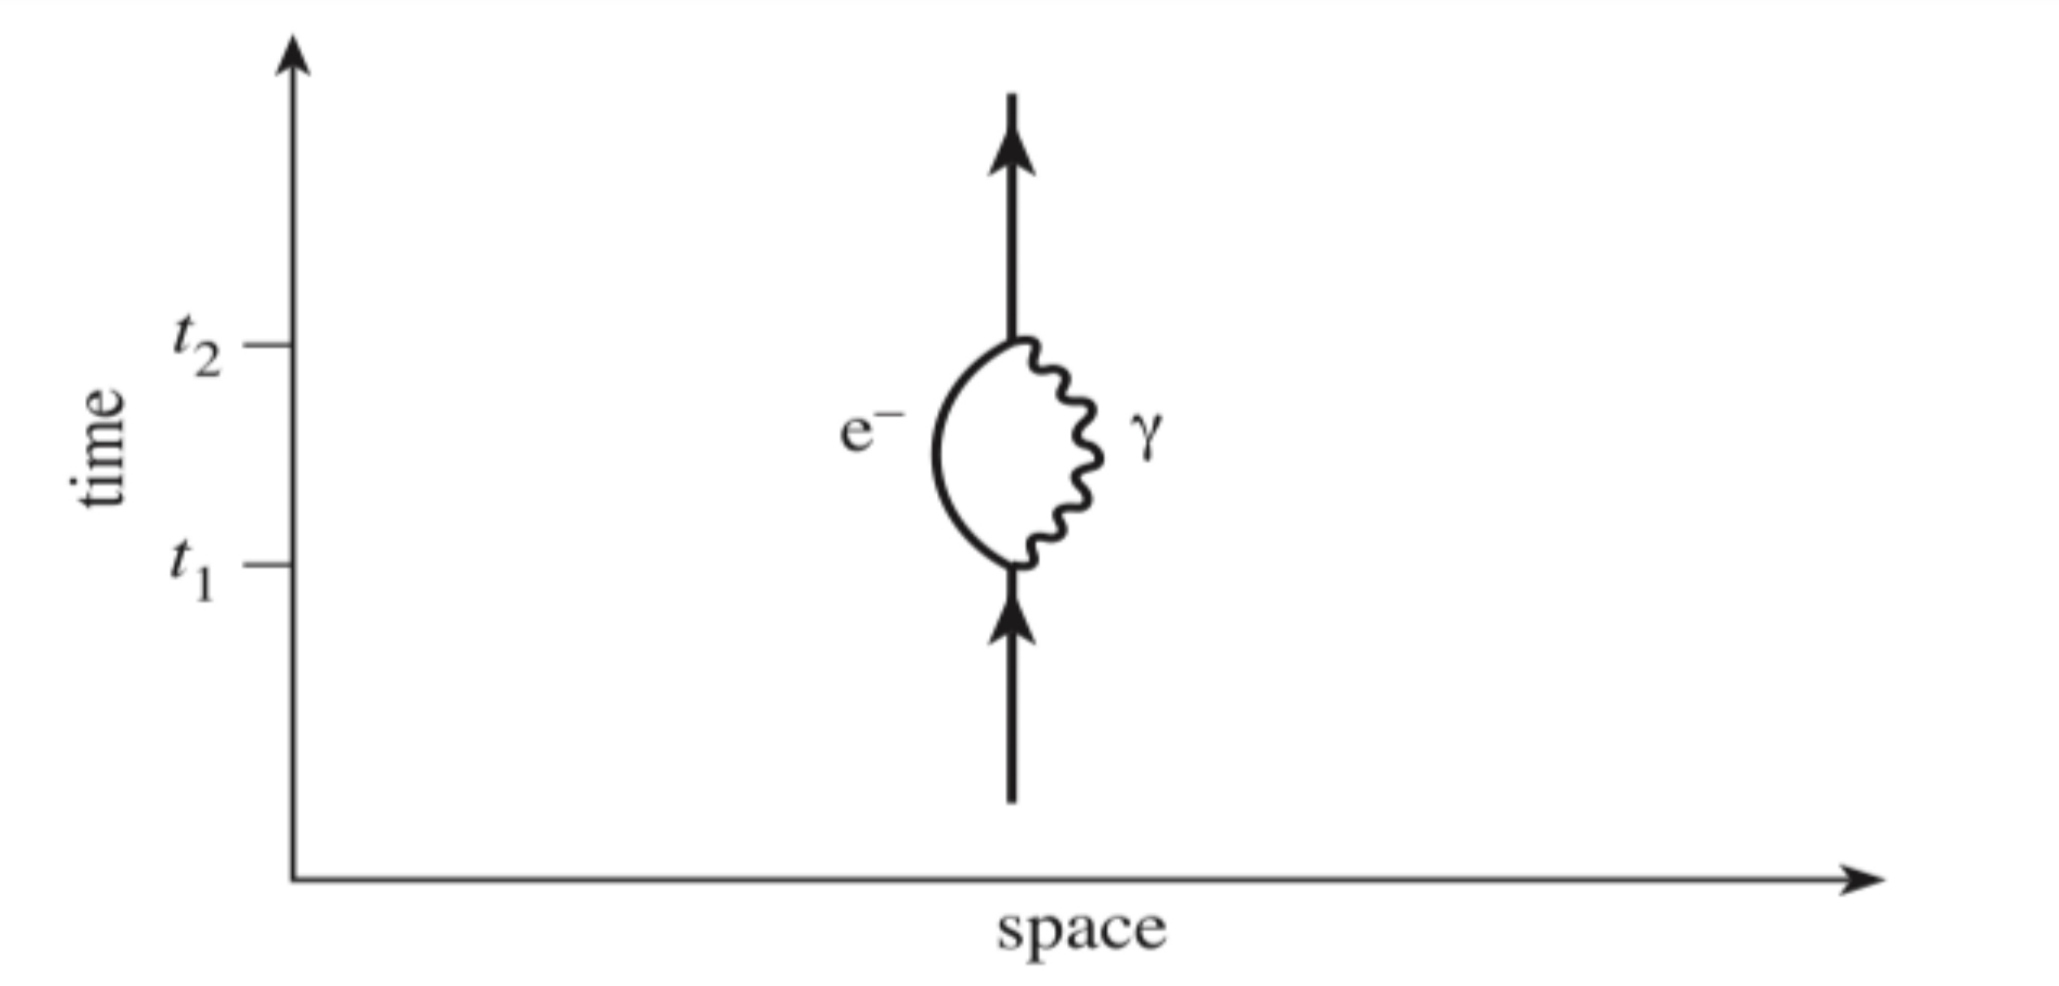
\includegraphics[scale=0.10]{02/img1.jpg}
            \end{center}
            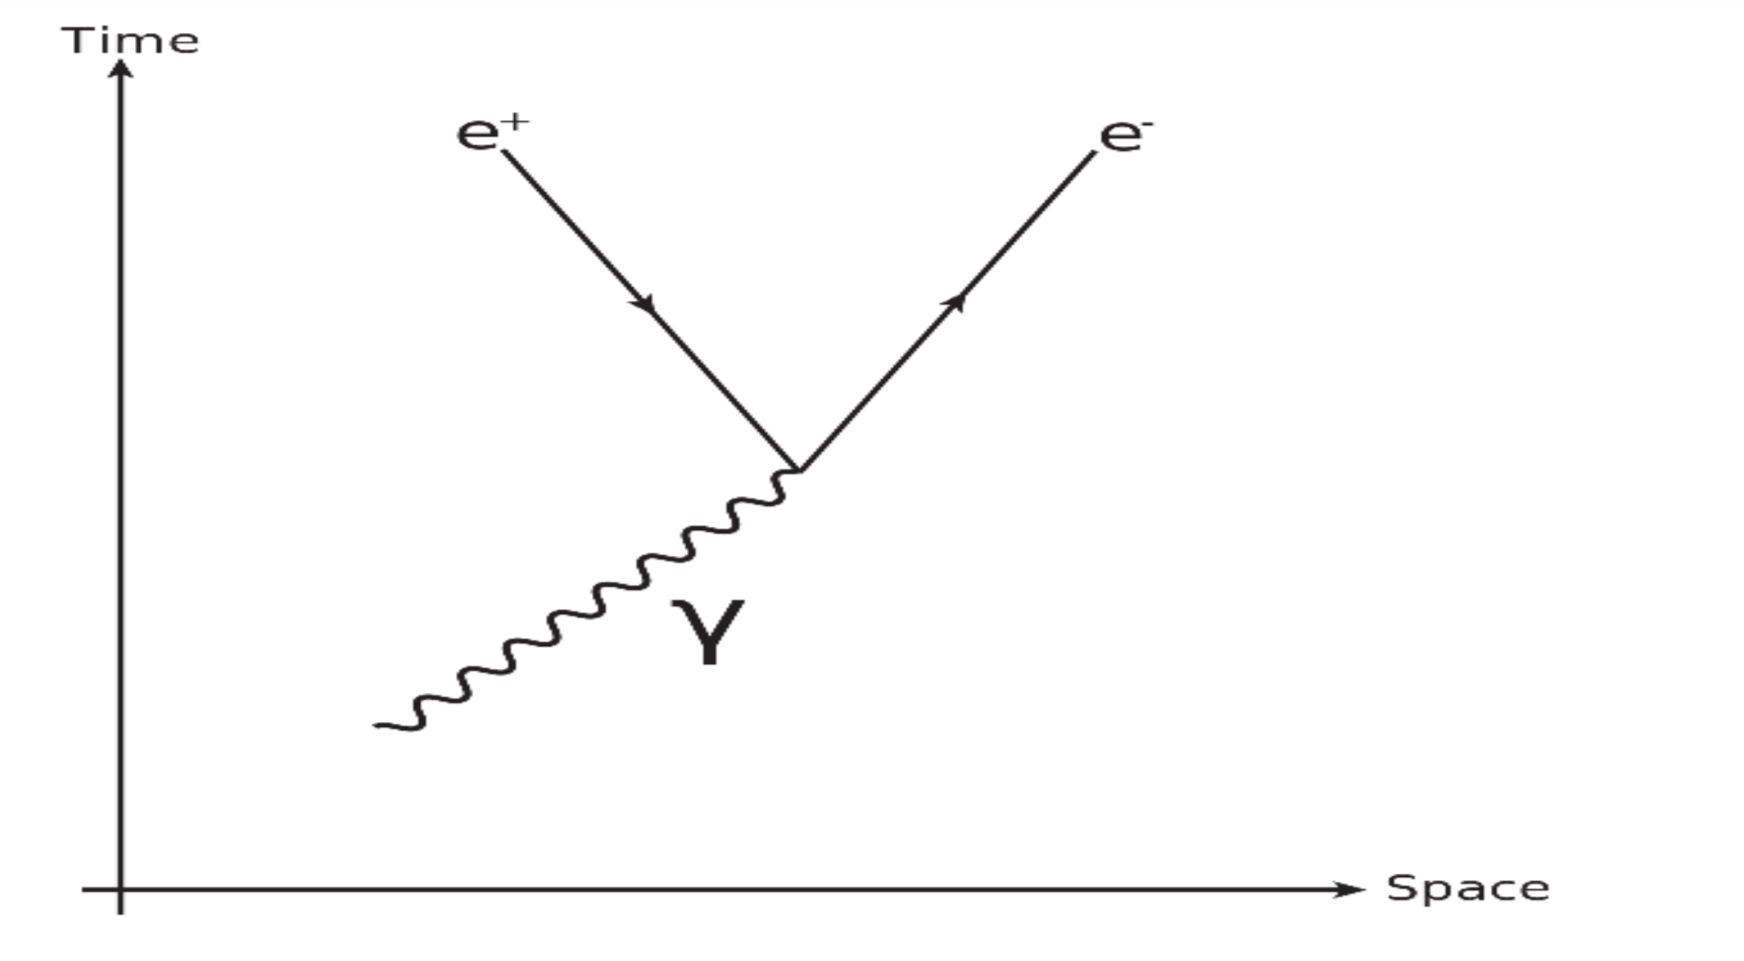
\includegraphics[scale=0.10]{02/img2.jpg}
            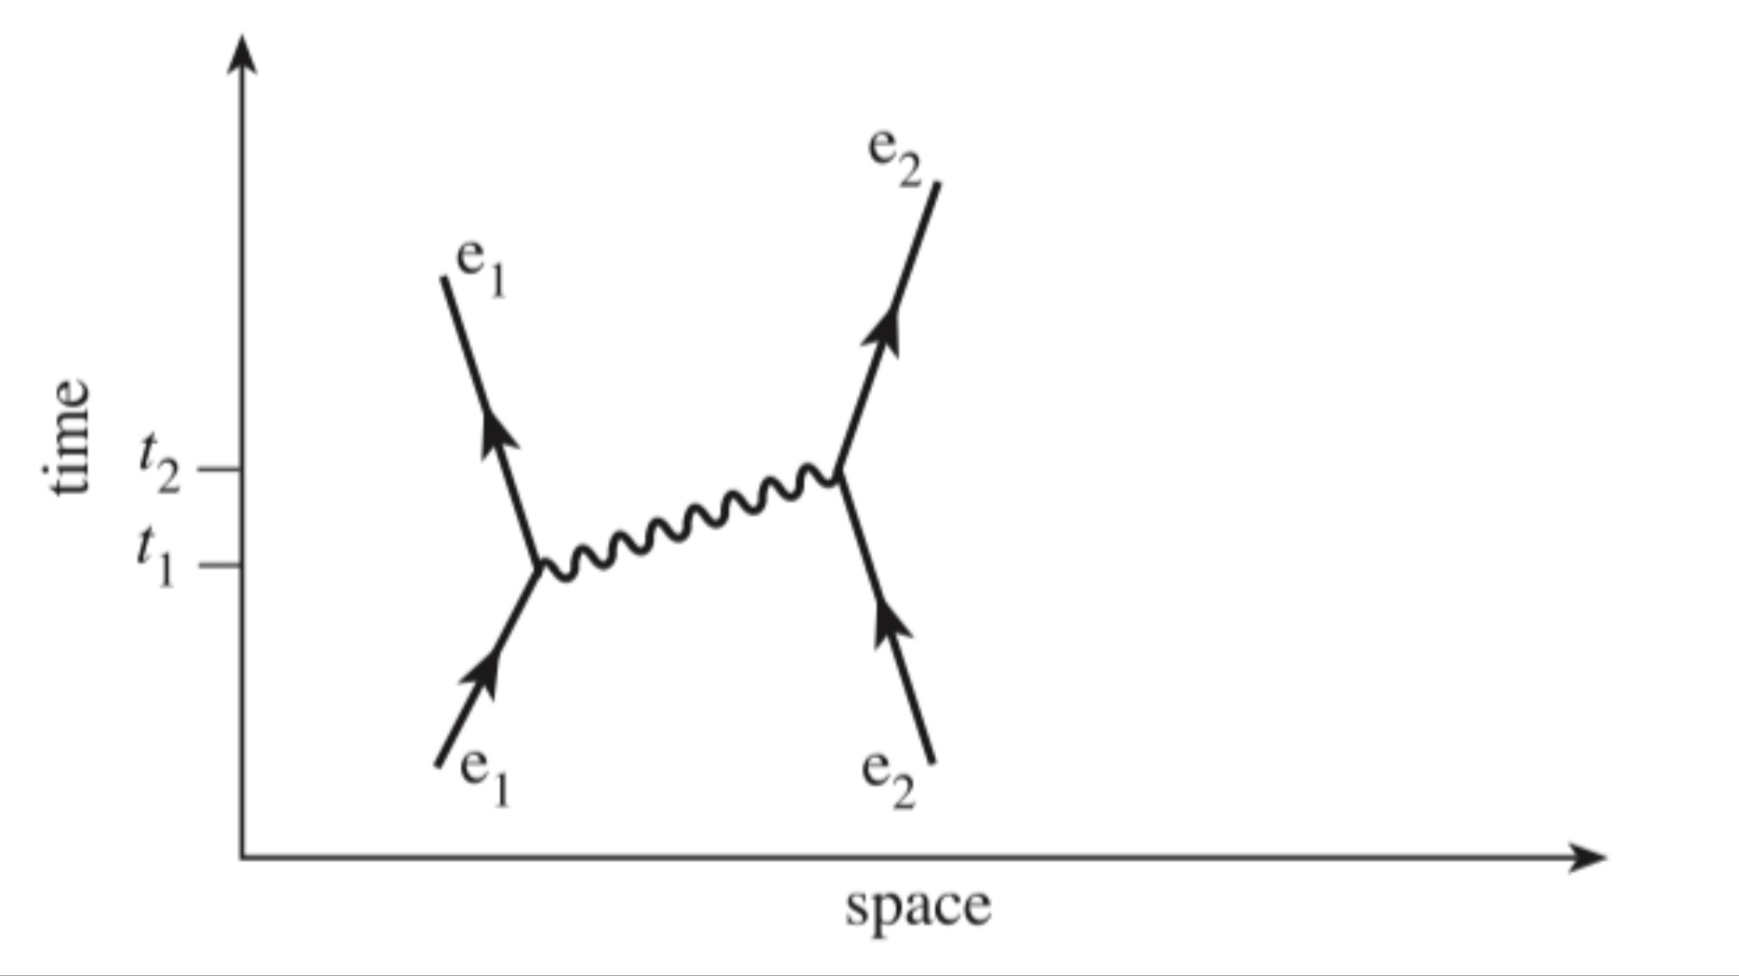
\includegraphics[scale=0.10]{02/img3.jpg}
            \caption{Feynman diagrams}
            \label{fig:plot_time_space}
        \end{figure}
        and once again absorbed at $t_2$. Similarly, the process of pair production can be represented by the above diagram. Note that the arrow of an anti-particle will be drawn backwards in time (opposite of particle). Two electrons scattering may be represented by the following figure:  At $t_1$, electron $e_1$ emits a virtual photon and to conserve momentum it will recoil to the left. At $t_2$ ($<\Delta t$), $e_2$ absorbs the photon and deflects to the right to conserve momentum. In addition, the total energy of the two–electron system should remain the same before and after the scattering to satisfy the energy conservation principle.
